\chapter{Evaluation of the ML-Based Reconstruction}
\label{chap:performance-evaluation}
To evaluate the performance of the ML-based reconstruction method, several metrics and analyses are conducted. This chapter presents the results of these evaluations, focusing on the accuracy of particle assignments, the reconstruction of relevant physics variables, and the performance across different kinematic regions. For this evaluation, the ML-based methods are compared against the baseline reconstruction techniques. The comparison includes both the overall performance and the performance in specific regions of interest, such as near the $t\bar{t}$ production threshold. Furthermore, the impact of the improved reconstruction on the resolution of key observables is assessed, demonstrating the potential benefits for precision measurements and searches in top-quark physics.


\section{Machine Learning Metrics}
\label{sec:ml-metrics}


\section{Assignment Accuracy}
\label{sec:assignment-accuracy}
\begin{table}[ht]
    \centering
        \begin{tabular}{lcc}
        \toprule
        Method & Assignment Accuracy & Selection Accuracy \\
        \midrule
        $\Delta R(\ell,j)$-Method & $0.63455_{-0.00042}^{+0.00050}$ & $0.92333_{-0.00041}^{+0.00035}$ \\
        $\chi^2$-Method & $0.73896_{-0.00048}^{+0.00039}$ & $0.92329_{-0.00037}^{+0.00031}$ \\
        CompactTransformer & $0.8230_{-0.0006}^{+0.0005}$ & $0.95946_{-0.00036}^{+0.00024}$ \\
        \bottomrule
    \end{tabular}
    \caption{Comparison of assignment and selection accuracies for different reconstruction methods. The uncertainties represent the statistical variations in the evaluation dataset.}
    \label{tab:reconstruction-accuracies}
\end{table}
The assignment accuracy is defined as the fraction of events where the reconstructed particles are correctly assigned to their parent partons. The selection accuracy, on the other hand, measures the fraction of events where the correct assignment is among the selected candidates. Both metrics are crucial for evaluating the performance of reconstruction methods, as they directly impact the resolution of physics observables and the sensitivity of analyses. Furthermore, some variables, such as the invariant mass of the $t\bar{t}$ system, are only sensitive to the correct selection of candidates, making the selection accuracy particularly important for certain analyses. The \Cref{tab:reconstruction-accuracies} summarises the overall assignment performance of the reconstruction methods.
The ML-based method, represented by the CompactTransformer, shows a significant improvement in the assignment accuracy compared to the $\Delta R(\ell,j)$-Method and the $\chi^2$-Method. The improvement for the selection accuracy is rather small, which can be attributed to the b-tagging. Because baseline methods almost exclusively rely on b-tagging for the selection, and the GN2-tagger is very performant \cite{gn2_btagger}, the selection accuracy is already very high. Further, the b-tagging of the GN2-tagger already takes into account the full kinematic information of the event, making it difficult for the ML-based method to significantly outperform the selection accuracy.
Regarding the assignment accuracy, the ML-based method shows a significant improvement, which can be attributed to its ability to learn complex correlations between the kinematic variables of the reconstructed particles.\\
\begin{figure}[ht]
    \centering
    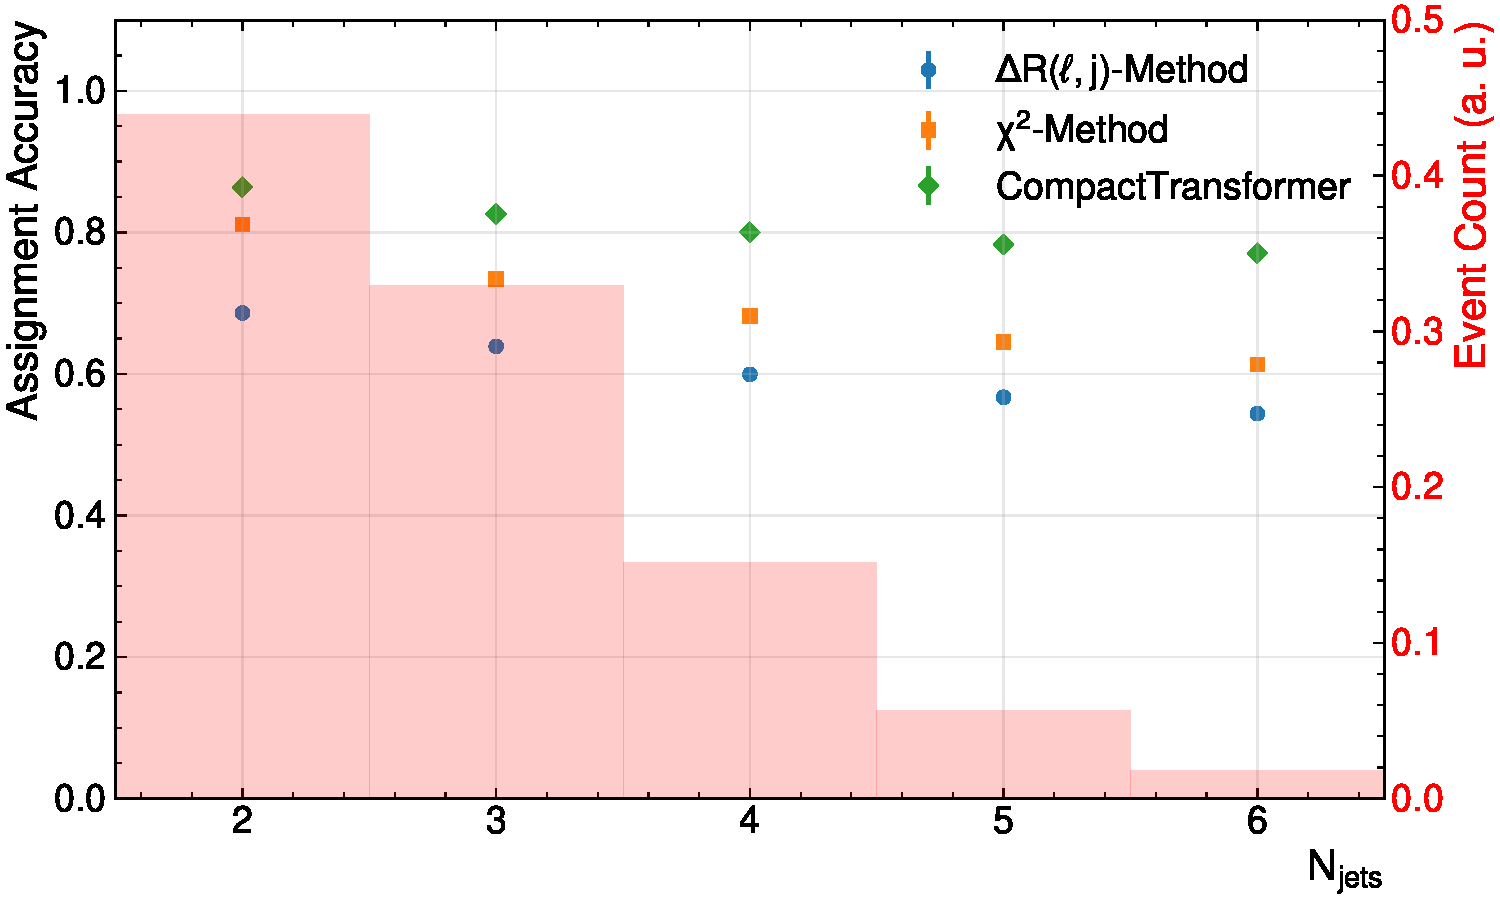
\includegraphics[width=0.7\textwidth]{plots/compact_assigner/binned_performance/N_jets/binned_accuracies_N_jets.pdf}
    \caption{Assignment accuracy as a function of the number of jets in the event for different reconstruction methods. The background histograms show of the distribution of events as a function of the number of jets. The uncertainties represent the statistical variations in the evaluation dataset.}
    \label{fig:accuracy_vs_njets}
\end{figure}%
The \Cref{fig:accuracy_vs_njets} shows the assignment accuracy for different jet multiplicities for the different methods. It can be observed, that the CompactTransformer outperforms the baseline-methods in all bins. For all methods, the performance drops with an increasing number of jets. The performance drop, however, is relatively small, which can be attributed to the performance of the b-tagging. Notably, the performance of the CompactTransformer drops the least, and the difference in performance increases for higher jet numbers. This stems from the improved accuracy of the jet-selection as shown before. In the Appendix, the \Cref{fig:selection_accuracy_vs_n_jets} shows the selection accuracy binned in the same way. It can be seen that the CompactTransformer does a much better job at selection the correct jets for events with a higher jet multiplicity. It was found, that this is the primary cause for differences in assignment accuracy with respect to the jet-multiplicity. The efficiency of assigning correctly selected jets seems to be mostly independent of the jet-multiplicity.
\begin{figure}[ht]
    \centering
    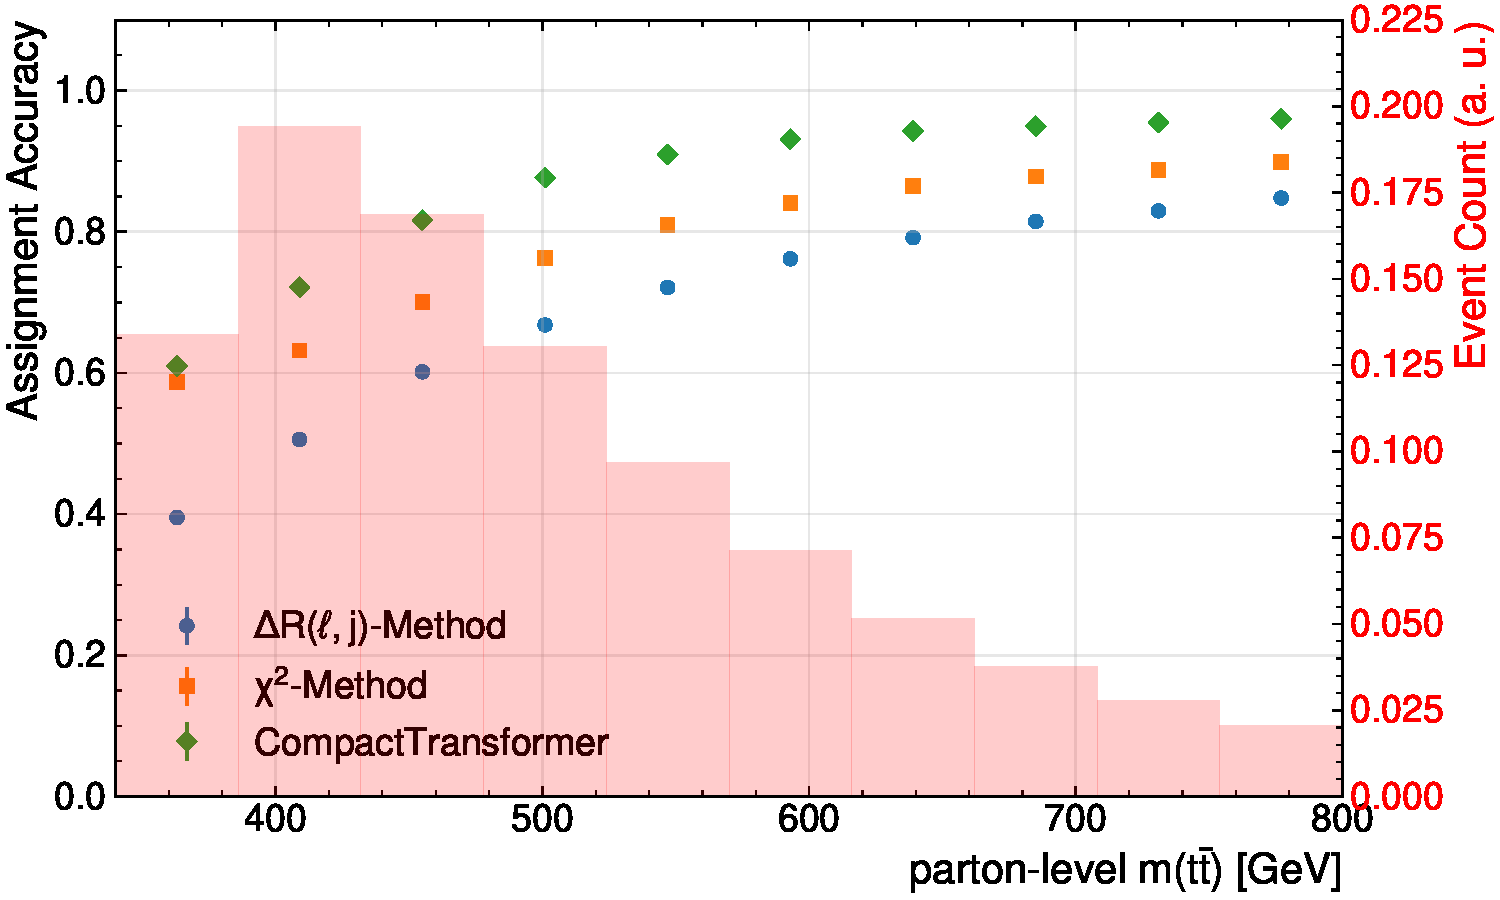
\includegraphics[width=0.7\textwidth]{plots/compact_assigner/binned_performance/truth_ttbar_mass/binned_accuracies_truth_ttbar_mass.pdf}
    \caption{This plot shows the assignment accuracy in bins of the true invariant mass of the top-quark pair.}
    \label{fig:accuracy_vs_mttbar}
\end{figure}
\Cref{fig:accuracy_vs_mttbar} shows the assignment accuracy as a function of the parton-level $m(t\bar{t})$. All methods show a similar behaviour; the accuracy drops for low invariant masses and seems to saturate for high invariant masses. For the CompactTransformer, the saturated performance in the high invariant mass regime almost approaches unity, marking near perfect reconstruction. On the other end of the spectrum, the performance drops to around 0.6 near the \ttbar-production threshold. For these low-mass events, the CompactTransformer and the $\chi^2$-Method appear to be almost on-par. In general, this indicates that the $\chi^2$-Method is the leasts sensitive to $m(t\bar{t})$, while the $\Delta R(\ell,j)$-Method seems to be most sensitive. One can consider the conditional probability to make a correct assignment, given that the correct jets were selected. For this situation, the assignment reduces to a binary problem in the dilepton case, as jets can only be assigned to bottom- or antibottom-quark respectively. According to the Bayes' theorem, this probability can be computed by dividing the assignment accuracy with the selection accuracy.
\begin{figure}[ht]
    \centering
    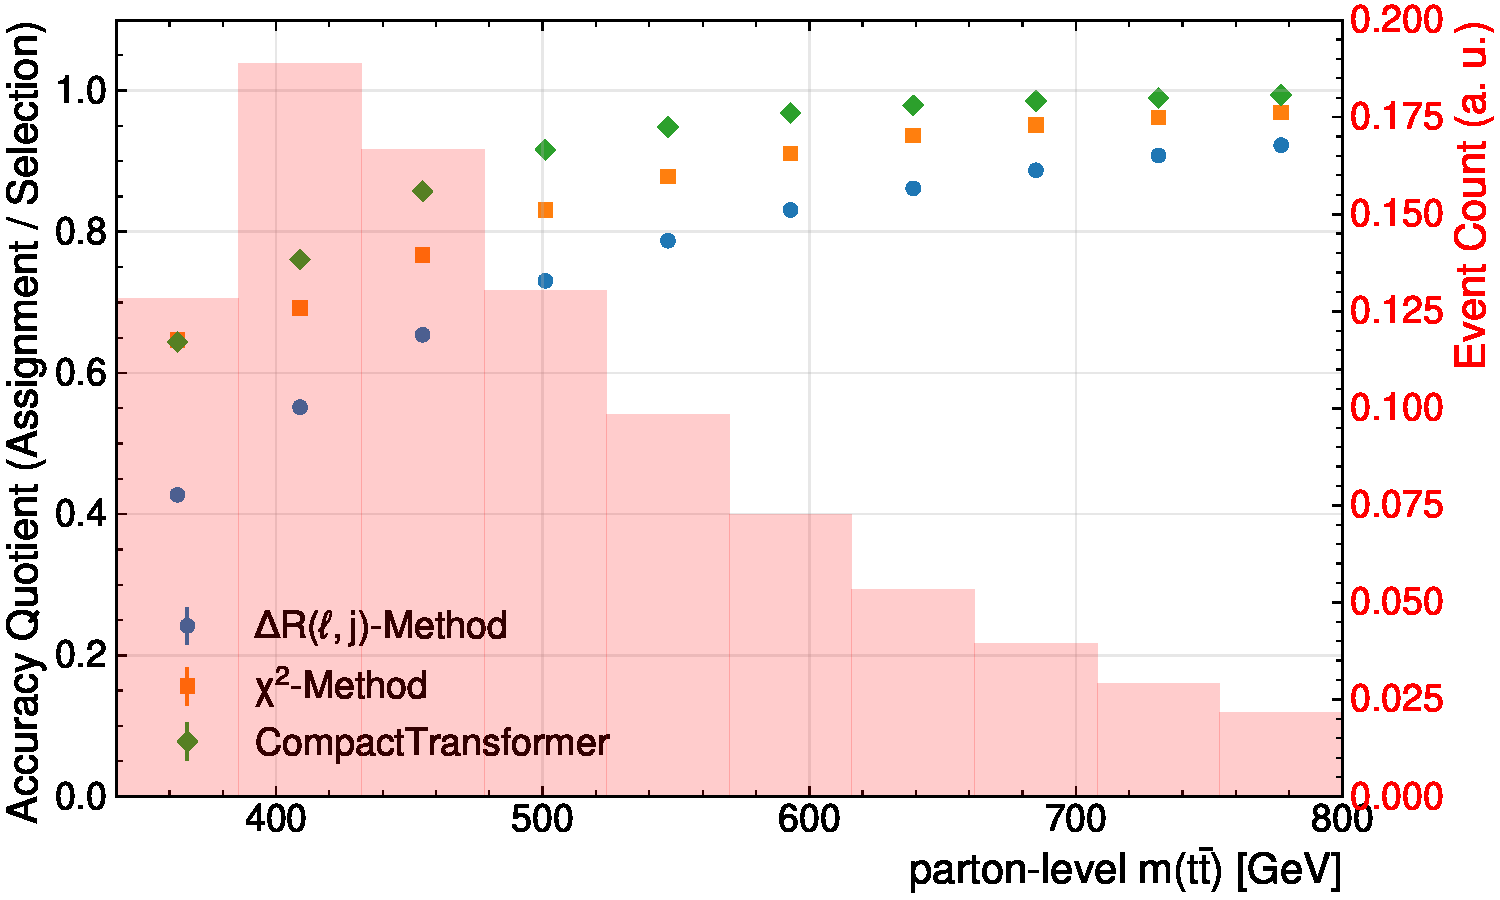
\includegraphics[width=0.7\textwidth]{plots/compact_assigner/binned_performance/truth_ttbar_mass/binned_accuracy_quotients_truth_ttbar_mass.pdf}
    \caption{Quotient of assignment and selection accuracy computed in bins of the parton-level $m(t\bar{t})$.}
    \label{fig:accuracy_quotient_vs_mttbar}
\end{figure}
The corresponding plot showing this probability for the different methods, binned in parton-level $m(t\bar{t})$, is displayed in \Cref{fig:accuracy_quotient_vs_mttbar}. This investigation allows to separate the process of actually assigning the selected jets. One thing one to note, is that the $\Delta R(\ell,j)$-Method has a performance below $0.5$ for the lowest bin, meaning that it performs worse than a random assignment in this bin. This suggests, that the topology of the particles in this region actually disfavours assigning jets based on proximity. \Cref{fig:deltaR_pairing} in the Appendix clearly shows the difference in angular distance for correct and incorrect jet-lepton pairing between the inclusive sample and the near-threshold region.
Another observation is, that in the lowest bin, the CompactTransformer and $\chi^2$-Method are completely on par for this metric. Generally, it can be concluded, that the region close to the production threshold features a particularly challenging topology for the assignment of jets. One particular property of the events close to the production-threshold is, that they feature smaller separation of the leptons. The double-binned distribution of events in \Cref{fig:feature_2d_mttbar_dR_l1l2} shows that events with lower $m(t\bar{t})$ tend to have more collimated leptons, whereas they are more separated for more energetic events.
Since the angular separation of the leptons is suspected to worsen the performance of the events, its impact on the individual methods is investigated.
\begin{figure}[ht]
    \centering
    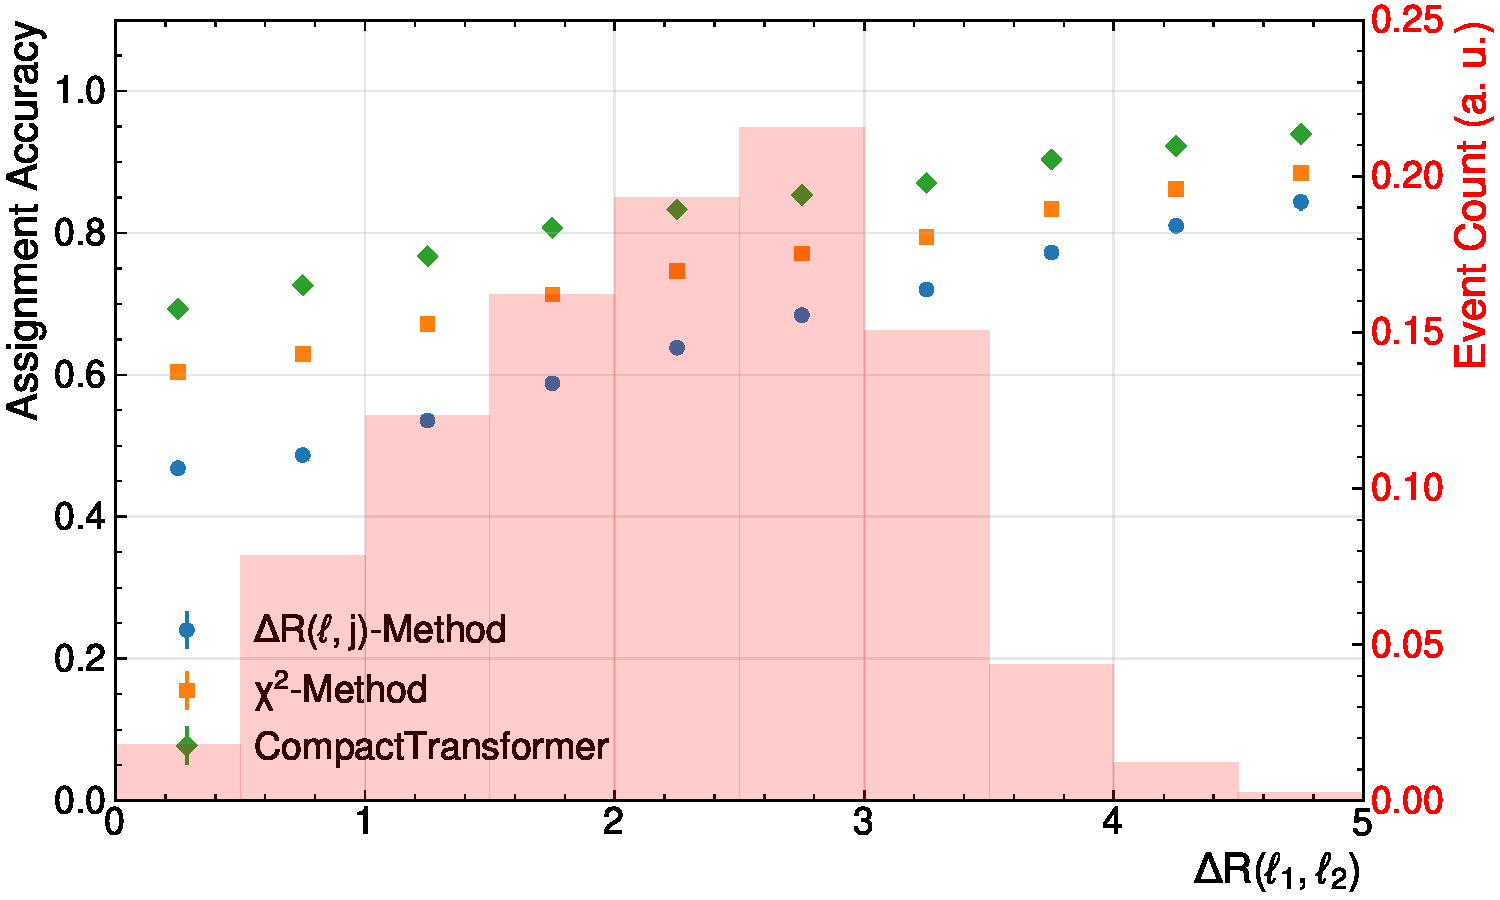
\includegraphics[width=0.7\textwidth]{plots/compact_assigner/binned_performance/dR_l1l2/binned_accuracies_dR_l1l2.pdf}
    \caption{Assignment accuracy binned in the angular distance between the two leptons of the events $\Delta R(\ell_1,\ell_2)$.}
    \label{fig:accuracy_vs_dr_l1l2}
\end{figure}
\Cref{fig:accuracy_vs_dr_l1l2} shows the assignment accuracy in bins of the angular distance $\Delta R(\ell_1,\ell_2)$ between the two leptons. All methods suffer losses in performance for events with close leptons. Interestingly, however, even for the smallest\footnote{Due to the so-called overlap-removal, which removes overlapping objects from the events, there is a cut-off at $\Delta R<0.3$. This technique accounts for the fact that in a detector objects that coincidence cannot be separated.} angular separation the performance is still above the one for near-threshold events.
A combined comparison of both variables' impact is shown in \Cref{fig:accuracy_2d_mttbar_dR_l1l2} in the Appendix. The double-binned accuracy reveals, that the invariant mass $m(t\bar{t})$ seems to have a much stronger impact on the performance, than the angular separation alone.



\section{Neutrino Regression}
\label{sec:neutrino-regression}



\section{Variable Reconstruction}
\label{sec:variable-reconstruction}



\section{Region Specific Performance}
\label{sec:region-specific-performance}



